\chapter{Konzeption der Lösung}
\label{kap4}

\begin{figure}[b!]
  \centering
  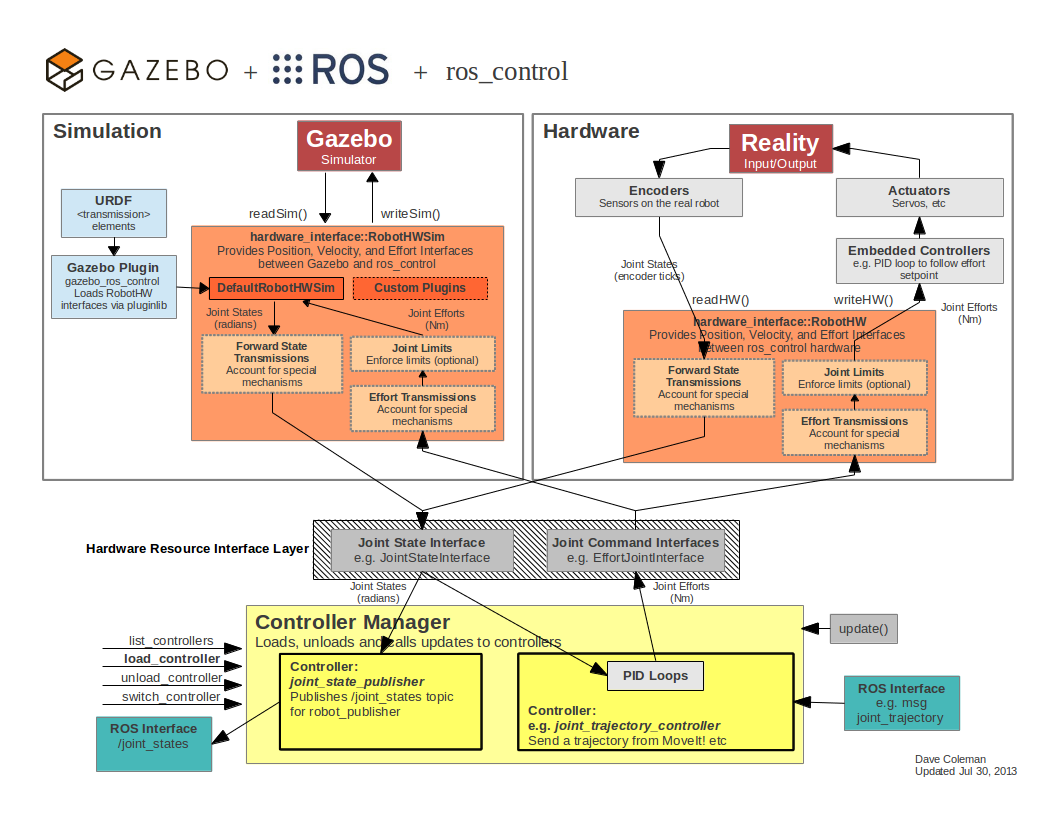
\includegraphics[width=\linewidth]{kapitel4/architecture}
  \caption[Architektur der Lösung mit Gazebo, \ac{ROS} und ros\_control]{Architektur der Lösung mit Gazebo, \ac{ROS} und ros\_control \autocite{chitta2017ros_control}}
  \label{Kap4:architecture}
\end{figure}

Dieses Kapitel nutzt die in \autoref{kap3} dargestellten verwandten Arbeiten, um ein Konzept für die Portierung des Laufplaners für den Akrobat in \ac{ROS} und Gazebo formal darzustellen. Als Basis dafür werden die Arbeiten von André Herms \autocite{herms2004} und Uli Ruffler \autocite{ruffler2006} herangezogen.

\autoref{Kap4:architecture} stellt die Architektur der Lösung dar. Diese besteht aus drei wesentlichen Bausteinen:
\begin{itemize}
\item Simulation: Gazebo
\item Hardware
\item \ac{ROS} mit dem Package ros\_control
\end{itemize}

Auf dem \ac{ROS} läuft der Laufplanungsalgorithmus, damit dieser sowohl für die Simulation als auch für die echten Hardware ausgeführt werden kann. Die Abstraktion zwischen Gazebo bzw. der echten Hardware und \ac{ROS} ist sinnvoll, da so im späteren Verlauf des Projekts einfach auf die echte Hardware gewechselt werden kann. Dies liegt daran, dass die Schnittstellen dann die selben sind. Auch das im Hintergrund laufende \ac{ROS} führt die gleichen Berechnungen wie sonst auch aus.

Die nächsten beiden Abschnitte gehen nun genauer auf die Simulationsumgebung Gazebo und deren Schnittstelle zu \ac{ROS} ein sowie auf die Lösung der Laufplanung ein.

\section{Simulationsumgebung Gazebo} 

Um die reale Umgebung zu simulieren, benötigt die Lösung eine Physik-Engine, die bei André Herms \autocite{herms2004} Simulationsumgebung nur rudimentär vorhanden ist. Bei der Nutzung von Gazebo wird standardmäßig die \acf{ODE} mitgeliefert, welche auch hierbei zum Einsatz kommen soll.

Zusätzlich soll es möglich sein, verschiedene Umgebungen laden zu können, damit die Flexibilität beim Testen der Laufalgorithmen erhalten bleibt. Dies ist mit Hilfe von verschiedenen Gazebo-Welten zu lösen. Im ersten Schritt soll dazu eine leere Welt genutzt werden.

Um außerdem ein möglichst reales Szenario zu simulieren, muss ein präzises Robotermodell im Format \ac{URDF} für das \ac{ROS} und Gazebo zum Einsatz kommen, welches das Aussehen, das Kollissionsmodell sowie die Massenträgheit genau beschreibt. Der bestehende Laufplaner besitzt aktuell noch das Modell des \emph{Lauron III}, welches in der neuen Lösung keine Anwendung mehr findet.

Des Weiteren sollen die Gelenkbewegungen nicht mehr über OpenInventor \autocite{inventor} ausgeführt werden. Dazu soll ein \ac{ROS}-spezifisches Paket mit dem Namen \emph{ros\_control} verwendet werden. Durch dieses werden Motoren an den Gelenken simuliert, welche über \ac{ROS}-Topics angesteuert werden können.

\section{Laufplanung im \ac{ROS}}

Da der Laufplaner und die Simulation voneinander getrennt sein sollen, damit das System flexibel für den Austausch von Komponenten bleibt, benötigt der Laufplaner ebenso wie bei André Herms und Uli Ruffler eine xml-Schnittstelle, welche Bewegungen repräsentiert. Die hier dargestellte Schnittstelle soll eine Abwandlung der vorherigen Schnittstellen sein, da diese nicht die Dauer von Bewegungen speichert, sondern lediglich für jeden Schritt die Fußpositionen relativ zur definierten Ausgangsposition. Wie im Vorgängermodell sollen Bewegungen generiert und auch eingelesen werden können.

Der vorherige Laufplaner hat kinematische Berechnungen manuell in OpenInventor durchgeführt. Das neue System soll das \ac{ROS}-Framework \textsc{tf} verwenden, um möglichst einfach Koordinatentransformationen zu berechnen. Die inverse Kinematik wird weiterhin über die analytische Methode berechnet. Allerdings werden dabei die Objektfunktionen von \textsc{tf} verwendet. Weitere geometrische Berechnungen werden ebenfalls über das \textsc{tf}-Framework berechnet.

Des Weiteren muss der Algorithmus auf den Laufroboter Akrobat angepasst werden, da der vorherige Algorithmus auf dem \emph{Lauron III} basiert und die Maße andere sind.